\providecommand{\main}{..}
\documentclass[\main/thesis.tex]{subfiles}

\onlyinsubfile{\zexternaldocument*{\main/tex/main chapter}}


\definecolor{codegreen}{rgb}{0,0.6,0}
\definecolor{codegray}{rgb}{0.5,0.5,0.5}
\definecolor{codepurple}{rgb}{0.58,0,0.82}
\definecolor{backcolour}{rgb}{0.95,0.95,0.92}


\lstdefinestyle{code_snippet_style}{
    backgroundcolor=\color{gray!10},
    basicstyle=\footnotesize\ttfamily,
    commentstyle=\color{codegreen},
    keywordstyle=\color{magenta},
    breakatwhitespace=false,
    breaklines=true,
    captionpos=b,
    keepspaces=true,
    numbers=left,
    numbersep=5pt,
    numberstyle=\tiny\color{gray},
    showspaces=false,
    showstringspaces=false,
    showtabs=false,
    tabsize=2
}


\lstset{
    style=code_snippet_style,
    columns=fullflexible,
    basicstyle=\ttfamily,
    frame=tlbr,
    postbreak=\mbox{\textcolor{red}{$\hookrightarrow$}\space},
    breaklines=false,
    framerule=0pt,
    framexleftmargin=0pt,
    framexrightmargin=0pt,
    framexbottommargin=1pt,
    aboveskip=10pt,
    belowskip=10pt,
    xleftmargin=0.01cm,
    xrightmargin=0.01cm
}


    

\begin{document}


\chapter{Backgrounds}

Single Instruction Multiple Data or SIMD instructions are used by processors to make computations faster as they execute the same operation on multiple data simultaneously. Using these instrcutions typically leads to a significant performance improvement as a result, compiler specialists try to explore different ways to utilize these instrcutions. Auto-vectorization [cite] is the most popular approach to use SIMD instrcutions in modern compilers. It's a compiler tranformation that tries to replace scalar code  (i.e., simple instructions) with SIMD instrcutions whenever it finds it both possible and beneficial. For this reason, these set of instrcutions are also called vector instrcutions.
In majority of applications, most of the execution time is spent on loops as a result, although there are works thhat try to aply vectorization on different regions of code such as funtion [cite], it is typically applied on loops. To do this, modern compilers are equipped by optimization passes such as slp-vectorizer in Clang compiler [cite] to automatically do the tranformation.

%%%%%%%%%%%%%%%%%%%%%%%%%%%%%%%%%%%%%%%%%%%%%%%%%%%%%%%%%%%%%%%%%%%%%%%%%%%%%%%%%%%%%%%%%%%%%%%%%%%%%%%%%%%%%%%%%%%%%%%%%%%%%%%%%%%%%%%%%
% Modern processors utilize Single Instruction Multiple Data (SIMD) instructions to execute the same instruction on multiple data simultaneously. This technique provides significant performance improvements, leading compiler specialists to explore different ways to exploit SIMD instructions. One of the most popular approaches is auto-vectorization [cite], a compiler transformation that looks for opportunities to use SIMD instructions (also known as vector instructions) in a program and replaces scalar code (i.e., simple instructions) with vector instructions whenever possible. This transformation is implemented by almost all current compilers.
% Since most of the execution time of a program is spent on loops, vectorization is typically applied to loops. Well-known compilers have optimization passes, such as the slp-vectorizer in Clang [cite], that vectorize loops' bodies. Although there have been efforts to vectorize other structures, such as functions [cite], the primary focus of research in this area is on loops.

A considerable amount of work has been done to improve code using vectorization [cite]. However, this transformation requires the code to meet certain requirements; otherwise, compilers may produce invalid code. Moreover, replacing scalar code with vector instructions is not always beneficial. In some cases, scalar code can provide better performance than vector code. To address these two issues, compilers include an analysis pass to check both the legality of the transformation and its profitability.
One of the significant obstacles for vectorization is control flow divergence. When a program contains branches (e.g., if-then-else or switch-case statements), it can take different paths during runtime based on certain conditions within the code that may change dynamically. This is called divergence in the control flow of the program. With control flow divergence, vectorization cannot be applied easily, as different iterations of the loop may take different paths, disabling the compiler from replacing instructions with SIMD ones.
To tackle control flow divergence, a transformation called If-Conversion (also known as Control Flow Linearization) has been proposed. Modern processors support "predicated instructions," in which each instruction is guarded by a one-bit predicate that can be either 1 or 0. The execution of the instruction will be committed only if the predicate bit is set to 1. Otherwise, the result will be discarded, leaving no architectural effects, such as memory writes, etc. With "Predicated Vector instructions" in the processor,
compilers can vectorize codes with divergence by first linearizing control flow and then replacing scalar instructions with vectorized ones. 
This is the most widely used approach to vectorize such codes with divergence. However, there are problems with this approach.

To demonstrate possible shortcomings with this approach, let's follow a simple example: 
\begin{lstlisting}[language=C, caption={Motivating Example}]
    for(i = 0; i < n; i++){
        if(cond[i]){
            a[i] = b[i] * c[i];
        }else{
            b[i] = a[i] + c[i];
        }
    }
\end{lstlisting}

This code contains an if-else statement inside the loop, causing control flow divergence. To vectorize this code, we first need to linearize the control flow by converting the if-else statement to a sequence of predicated instructions. After linearization, the resulting code would look like this (assuming a vector length of 4):


\begin{lstlisting}[language=C]
    VLength= 4;
    for(i = 0; i < n; i+=VLength ){
        a_v = load_v(&a[i], VLength);
        b_v = load_v(&b[i], VLength);
        c_v = load_v(&c[i], VLength);
        mask_v = load_v(&cond[i], VLength);
        mask_not_v = not_v(mask_v);
        mult_v = masked_mul(b_v, c_v, mask_v);
        masked_store_v(&a[i], mult_v, VLength, mask_v);
        add_v = maked_add(a_v, b_v, mask_v);
        masked_store_v(&b[i],add_v, VLength, mask_not_v);
    }
\end{lstlisting}

The process of applying if conversion involves eliminating all branches and instead guarding all instructions with predicates. For example, in the case of a simple if-then-else statement, the predicate for the else block instructions will be the negation of the predicates used for the if block instructions. This allows us to effectively compute the instructions for both blocks without the need for branching, enabling us to use vector instructions and produce more efficient code.

However, one downside of applying if conversion is that we may end up wasting half of vector lanes due to predication, as we are always executing code in both the if and else blocks. As shown in Figure [?], the green elements represent the vector lanes executing the then block, the blue ones represent the vector lanes executing the else block, and the gray elements show inactive lanes. Regardless of how predicates are distributed among the mask vector, we are always losing half of our computation power due to predication. This is particularly true when the number of instructions in both the then and else blocks are approximately the same, which is often the case.

Moreover, the problem of wasted computation power due to predication is further intensified when we have unbalanced conditions, where we execute one of the two blocks more than the other. In such cases, the effect of predication is even more pronounced, as we end up losing more computation power due to the large number of inactive lanes.

This issue has been studied for a while, and recent works (cite) have proposed solutions to address it. The main idea behind most of these solutions is to detect uniform true and uniform false paths.

A uniform path refers to the case where, for one vector iteration, all predicates are either true or false, which means that all iterations are going to execute one path (in our motivating example, either the then block or the else block). If such a uniform path is detected, we only need to introduce a path that corresponds to the block it's going to execute, where all instructions are vectorized but not predicated. This way, we can utilize the full vector capacity to execute code and avoid the excessive overhead introduced by predicated instructions.

However, the main challenge is how to detect uniform vectors. As we discussed earlier and saw in the example, predicated vectors are formed from branch conditions. The value for these conditions could be either static or dynamic. If the condition is static, the compiler can find its value at compile time and apply appropriate optimizations to produce the most performant code. However, in most cases, the condition can only be determined at runtime and could change on each iteration, making static approaches unable to detect uniformity.

\begin{figure}[t!]
    \centering
    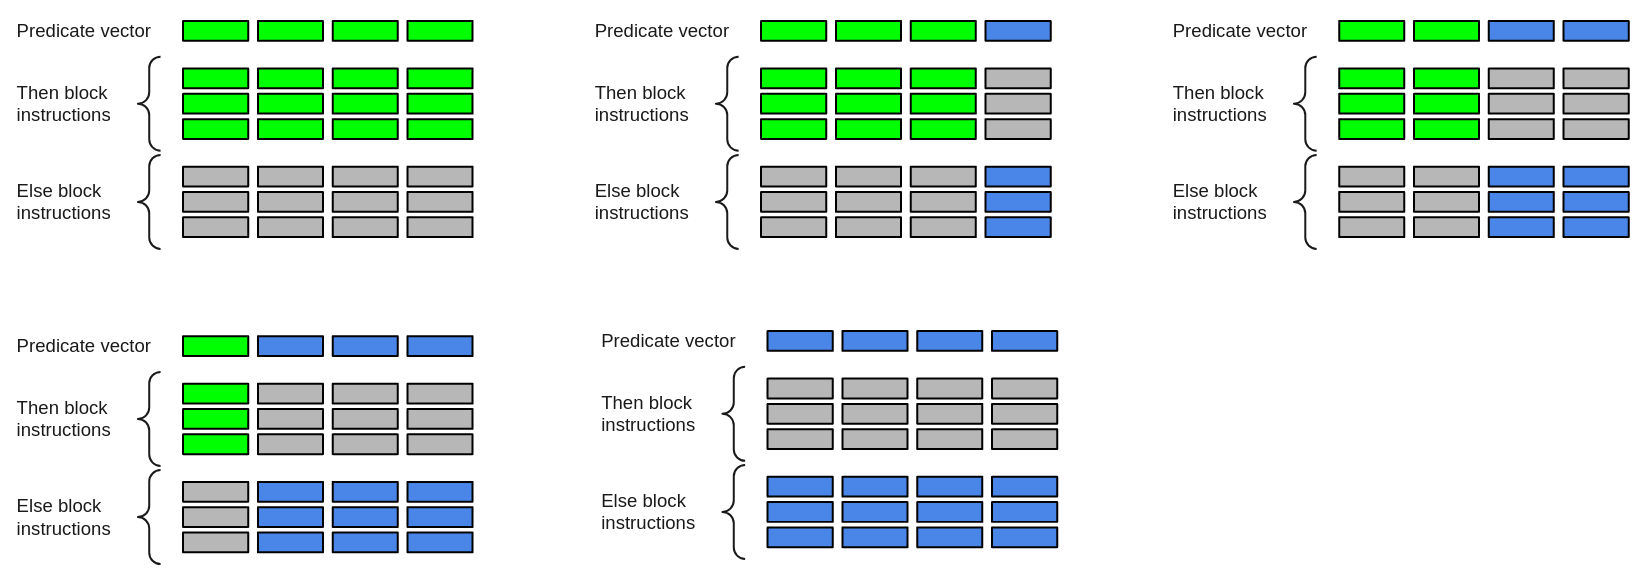
\includegraphics[width=1.1\textwidth, height=7.3cm]{img/condition_distribution.png}
    \caption{Wasting vector lanes due to predication}
    \label{fig:Permutation}
\end{figure}

Runtime checks are typical solutions to this problem. The compiler inserts some runtime checks to find out if a vector is uniform in that execution time or not. The compiler also introduces some paths so that when a uniform vector is detected dynamically, the corresponding path will be executed.

To demonstrate how this approach works, let's apply it on the code in figure [FIG number]:

\begin{lstlisting}[language=C]
    VLength= 4;
    for(i = 0; i < n; i+=VLength ){
        a_v = load_v(&a[i], VLength);
        b_v = load_v(&b[i], VLength);
        c_v = load_v(&c[i], VLength);
        mask_v = load_v(&cond[i], VLength);
        if(all_true(mask_v)){
            /* uniform true path */
            mult_v = b_v * c_v;
            store(&a[i], mult_v, VLength);
        } else if (all_false(mask_v)){
            /* uniform false path */
            add_v = a_v + c_v;
            store(&b[i],add_v, VLength);
        }else{
            /* Linearized Path */
            mult_v = masked_mul(b_v, c_v, mask_v);
            masked_store_v(&a[i], mult_v, VLength, mask_v);
            mask_not_v = not_v(mask_v);
            add_v = maked_add(a_v, b_v, mask_v)
            masked_store_v(&b[i],add_v, VLength, mask_not_v);
        }
    }
\end{lstlisting}

To avoid the performance overhead of predicated instructions, we need to detect if any uniform paths exist in the loop, where a uniform path is a sequence of instructions that always execute the same branch of the code based on a condition. To detect a uniform path, we first load the mask vector cond in line 6. We then check if all elements of the mask vector are true using the all\_true function in line 7. If this is the case, we have detected a uniform vector corresponding to the if block, and we can execute the if code without any predication. The if block consists of a multiplication of vectors b\_v and c\_v, and the result is stored in vector a\_v.

If all elements of the mask vector are false, we have detected a uniform vector corresponding to the else block. We can execute the else code without any predication. The else block consists of an addition of vectors a\_v and c\_v, and the result is stored in vector b\_v.

If some elements of the mask vector are true and others are false, it means that we have a combination of vectors that execute different paths in the code (some if block and some else). In this case, we use predicated code in our linearized path, as we did in the previous example.

Although uniform paths could potentially lead to performance improvements, there are two things to consider about them. First, they introduce overheads due to the runtime checks added to the code. Second, if the input data is such that uniform vectors are unlikely to occur, uniform paths won't be executed often, and no performance improvement will be gained. Therefore, the performance gains from the uniform path approach depend on the characteristics of the input data and the frequency of uniform vectors.



Wytte[cite] has proposed an innovative approach to overcome the problem of waiting for uniform vectors to occur, by suggesting the formation of such vectors through the use of his transformation called Active-Lane-Consolidation (ALC). The ALC transformation dynamically forms uniform vectors by permuting loop indices, thereby enabling the execution of the corresponding block without predication. The main idea behind this transformation is to create a uniform vector of indices that can execute the corresponding block of code without requiring any conditional statements.

This approach offers a more efficient and streamlined way of executing code, as it eliminates the need for predication and branching, which can result in slower execution times. By forming uniform vectors rather than waiting for them to occur, the ALC transformation helps the program to run more efficiently.

At the core of ALC is an algorithm named \emph{Permutation}, which aims to create a uniform vector with minimal overhead from two vectors and their corresponding predicates. The algorithm accomplishes this task by combining the input vectors in a specific manner. A high level view of the approach is shown in fig[?].

As can be observed, each input vector comprises a combination of true and false lanes, indicating the active and inactive values respectively. Following the permutation process, the resulting vector on the left-hand side contains only true lanes, while the other vector includes both active and inactive lanes. In this scenario, the permutation produces a uniform true vector. Regardless of the number of active and inactive lanes in the input vectors, there will always be at least one uniform vector, either true or false. Consequently, permuting loop indices allows us to execute one of the then or else blocks without the need for predication.


\begin{figure}[t!]
    \centering
    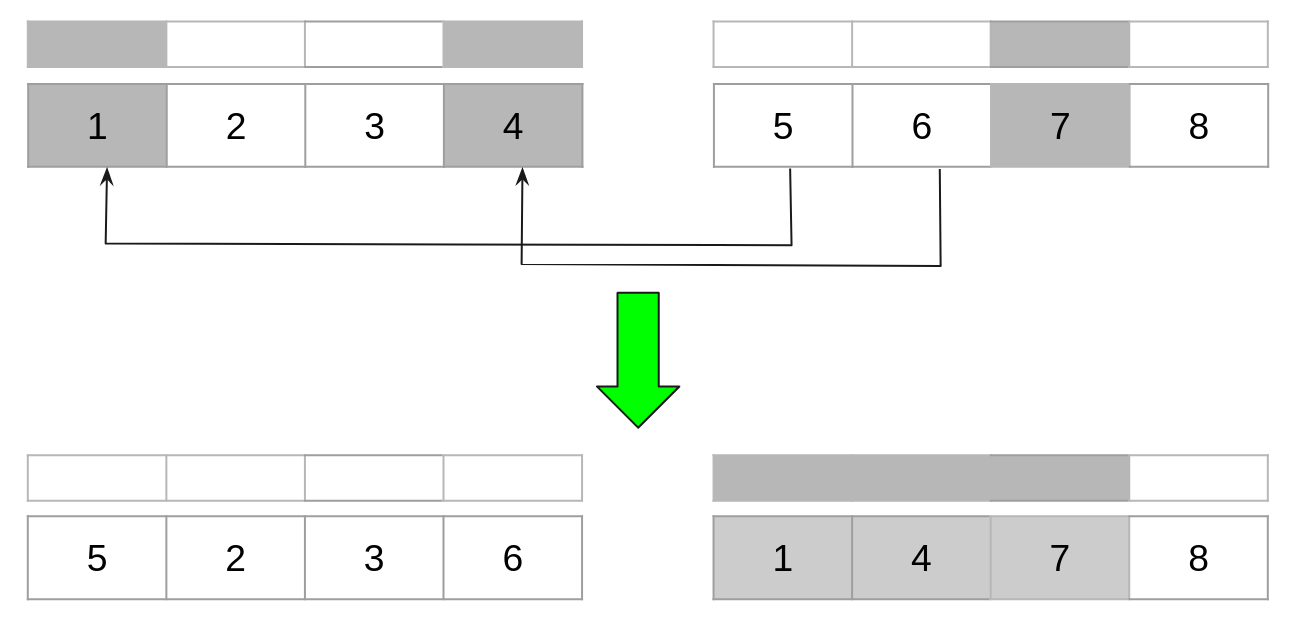
\includegraphics[width=0.95\textwidth]{img/permutation.png}
    \caption{Permutation}
    \label{fig:Permutation}
\end{figure}will

Being equipped by permutation, ALC can be implemented in our motivation code, as demonstrated in the following code snippet:

\begin{lstlisting}[language=C]
    VLength= 4;
    /*Initialization*/
    uniform_vec = index(0,VLength);
    uniform_mask = load_v(&cond[0], VLength);
    for(i = 0; i < n; i+=VLength ){
        index_vec = index(i, VLength);
        mask_vec = load_v(&cond[i], VLength);
        uniform_vec 
        ,remaining_vec
        ,uniform_mask
        ,remaining_mask =
        Permute(uniform_vec, index_vec, uniform_mask, mask_vec); 
                
        if(all_true(uniform_mask)){
            /* execute if block without predication */
            b_v = gather_load_v(&b, uniform_vec);
            c_v = gather_load_v(&c, uniform_vec);
            mul_v = b_v * c_v;
            scatter_store(&a, uniform_vec, mul_v);

            uniform_vec = remaining_vec;
            uniform_mask = remaining_mask;
        }else {     
            /* execute else block without predication */
            a_v = gather_load_v(&a, remaining_vec);
            c_v = gather_load_v(&c, remaining_vec);
            add_v = a_v + c_v;
            scatter_store(&b, remaining_vec, add_v);
        } 
    }
\end{lstlisting}

We can see how ALC is applied to our motivation code, starting with the initialization of the uniform vector (uniform\_vec) and its corresponding mask vector (uniform\_mask) in lines 3-4. These vectors are initialized with indices 0 to VLength and their corresponding masks, respectively.

In each iteration of the loop, the next vector of indices and its corresponding masked vector are formed (lines 6-7). The magic happens in line 11, where we call the permute function, which takes four input vectors: uniform\_vec, index\_vec, uniform\_mask, and mask\_vec. The function then arranges the active and inactive lanes of these vectors to form two output vectors: uniform\_vec (containing only active lanes) and remaining\_vec (containing inactive lanes and active lanes that were not included in the uniform\_vec). The function also generates two mask vectors, uniform\_mask and remaining\_mask, corresponding to the active and inactive lanes of the output vectors.

After calling the permute function, we check if all the mask bits in uniform\_mask are true (line 12). If this is the case, it means that we have formed a uniform vector corresponding to the then block, and we can execute it without the need for predication (lines 13-17). Specifically, we gather load the values of b and c vectors at the indices specified by uniform\_vec, multiply them, and store the result in the a vector at the same indices. We then update the uniform\_vec and uniform\_mask to reflect the active lanes that were not included in the uniform vector.

If all the mask bits in uniform\_mask are not true, it means that we have formed a uniform vector, corresponding to the else block. In this case, we can execute the else block without predication, as we know that all the mask bits in remaining\_mask are false (lines 18-22). We gather load the values of a and c vectors at the indices specified by remaining\_vec, add them, and store the result in the b vector at the same indices.

As we can see, by using ALC, we can always form a uniform vector (either uniform true or uniform false) in each iteration of the loop. This eliminates the need for predicated instructions and simplifies the code. Additionally, since the permute function generates uniform vectors, we can be confident that the code will execute correctly, without encountering any unexpected errors or behaviors.


Wytte proposed his transformation only for Arm SVE architecture. SVE (Scalable Vector Extension) is a vector extension proposed by ARM that is designed to address the limitations of existing vector unit extensions. One of the key features of SVE is that it supports very large vector lengths, up to 2048 bits. This allows for a higher degree of parallelism and makes it possible to process more data in a single instruction, which can result in significant performance gains.

Another powerful feature of SVE is its predication support. Unlike traditional vector extensions that have a single predicate register for the entire vector, SVE provides a vector of predicates for every vector of data. This allows for more fine-grained control over which elements of the vector are processed, enabling more efficient branching and reducing the need for predicated instructions.

In addition to its advanced predication support, SVE also provides a rich set of vector manipulation instructions that are optimized to move data between vector efficeintly. These instructions can efficiently rearrange the elements of a vector according to a specified pattern, making it possible to implement algorithms such as permutation with high efficiency.


\chapter{Main Chapter}


In this study, we build on the pioneering work of Wytte on the ALC technique. He first introduced the ALC idea and manually applied it to a few selected benchmarks, showing its potential to reduce the number of dynamically executed instructions compared to scalar and vectorized code. However, he conducted the experiments on a simulator since at the time, few machines supported SVE instructions.

While Wytte's results are promising, they do not provide sufficient evidence that ALC is actually beneficial. Vector instructions naturally reduce the number of executed instructions by processing multiple data at the same time, but they also introduce more overhead in terms of latency. Therefore, a careful evaluation of ALC is necessary to determine its effectiveness.

Another crucial aspect that could be severely impacted by the ALC transformation is memory access. When a load or store occurs, the processor also loads data from adjacent memory addresses into the cache, assuming that they will be used in the subsequent operations. This process, called locality, is essential for achieving good performance. However, ALC may alter the memory access pattern by using gather load and scatter store instructions to access different memory addresses. This change in behavior is likely to affect performance, but it cannot be easily detected through metrics such as executed instructions.

Thus, to assess the true impact of ALC, we need to consider different metrics including execution time and as well as the reduction in the number of executed instructions and the potential effects on memory access patterns. We conduct a thorough evaluation of ALC using a modern machine that supports SVE instructions and to compare its performance with that of scalar and vectorized code. Our evaluation provides insights into the effectiveness of ALC and help identify its potential limitations.




\section{Gather/Scatter Instructions}

This section delves into a comprehensive examination of gather load and scatter store instructions, which are commonly used in modern computer architectures. These instructions are designed to efficiently process data that is non-contiguous or has irregular memory access patterns, which can significantly impact the performance of memory-bound applications. By using gather load instructions, multiple memory locations can be accessed simultaneously and their contents combined into a single vector, reducing the number of memory accesses required. Conversely, scatter store instructions enable data to be written to non-contiguous memory locations simultaneously, which can further improve performance by reducing the number of memory write operations required.

While gather load and scatter store instructions can improve the performance of memory-bound applications, they also come with significant overhead. These instructions require additional hardware support and software optimizations to effectively utilize the parallelism inherent in the data access patterns. Additionally, the use of gather load and scatter store instructions can result in increased latency and less memory bandwidth utilization, which can negatively impact overall system performance.

\newpage

\begin{lstlisting}[language=C, caption=Scalar Code]
    for (int i = 0; i < n; i++) {
        if (cond[i]) {
            b[i] = a[i];
        }
    }
    \end{lstlisting}
    
    \begin{lstlisting}[language=C,caption=Vectorized Code]
        // predicate for all lanes true
        const svbool_t allActive = svptrue_b32(); 
        const int vl = svcntw(); // get vector length
        for (int i = 0; i < n; i += vl) {
            const svint32_t condVec = svld1_s32(allActive
                                                ,&cond[i]);
            // form predicate vector
            const svbool_t p_mask = svcmpeq_n_s32(allActive 
                                                  ,condVec
                                                  ,1); 
            const svint32_t a_vec = svld1_s32(p_mask, &a[i]);
            svst1_s32(p_mask, &b[i], a_vec); 
        }
    \end{lstlisting}
    
    \begin{lstlisting}[language=C,caption= Code Using Gather/Scatter]
        // predicate for all lanes true
        const svbool_t allActive = svptrue_b32(); 
        const int vl = svcntw();  // get vector length
        for (int i = 0; i < n - vl; i += vl) {
            indexVec = svindex_s32(i, 2);
            loaded = svld1_gather_s32index_s32(allActive
                                               ,a
                                               ,indexVec);
            svst1_scatter_s32index_s32(allActive
                                        ,b
                                        ,indexVec
                                        ,loaded);
    
        }
    \end{lstlisting}
    

\newpage

In order to gain a deeper understanding of how gather load and scatter store instructions work, we conduct a test to compare their performance with that of vectorized code. The scalar code used in the test is shown in the figure[?], which involves iterating over the array and copying elements from the input array to the output array only if the corresponding element in the condition array was true. The condition array is designed so that every other element was true, creating a non-contiguous and irregular memory access pattern.

To perform the test, we provide two versions of the code. The first is a vectorized version that utilizes masked instructions to perform loads and stores from consecutive memory addresses (figure[?]). The second version (figure[?]) utilizes gather load and scatter store instructions to load data from the addresses where we knew the corresponding condition is true. These addresses are computed at line 7 where we form a vecto of indices which corresponds to true elements.



\begin{figure}%
    \centering
    \subfloat[\centering Number of Program Cycles]{{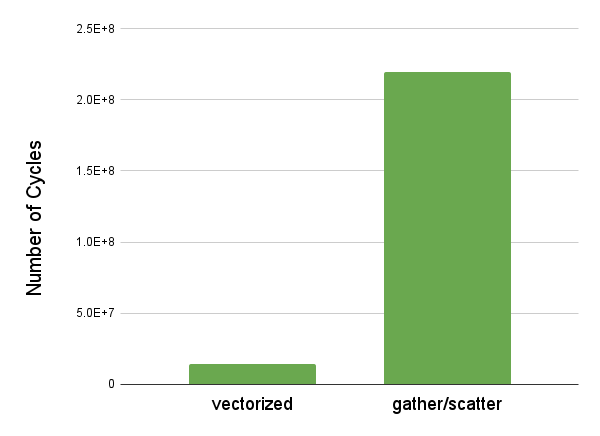
\includegraphics[width=6cm, height=5cm]{img/gather_scatter_cycles.png} }}%
    \qquad
    \subfloat[\centering Number of instructions executed]{{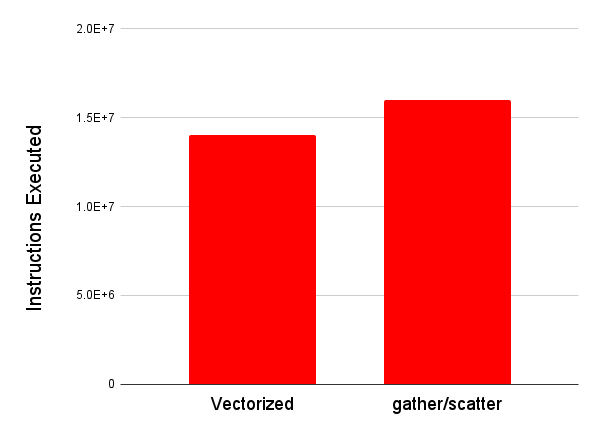
\includegraphics[width=6cm, height=5cm]{img/gather_scatter_instructions.png} }}%
    \caption{Comparison between Armclang vectorization and ALC}%
    \label{fig:example}%
\end{figure}

The comparison of the two versions of the code, as shown in Figure [?], reveals that there is a difference of less than 15\% in the number of executed instructions. However, the version that utilizes gather load and scatter store operations exhibits significantly poor performance, slowing down the program by more than 15x. This performance degradation is far greater than what could be accounted for by the mere 15\% increase in the number of dynamically executed instructions. Thus, additional metrics are necessary to better understand the underlying causes of this performance loss.

\begin{figure}[h]
    \centering
    \subfloat[Branch misses]{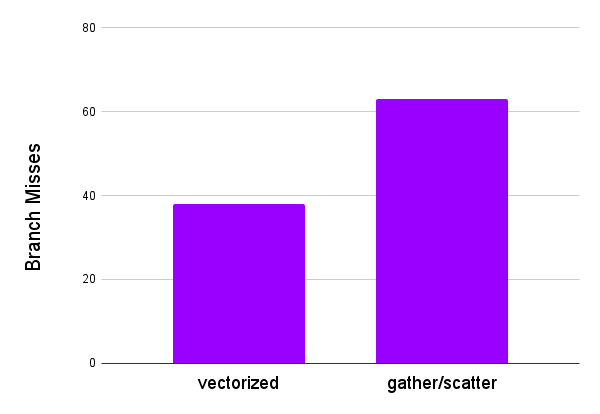
\includegraphics[width=0.5\textwidth]{img/gather_scatter_br_miss.png}}\hfill
    \subfloat[Cache misses.]{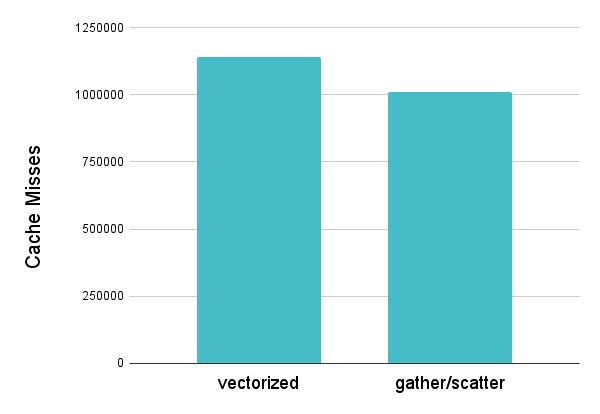
\includegraphics[width=0.5\textwidth]{img/gather_scatter_cache_miss.png}}\\
    \subfloat[Cycles stalled due to memory]{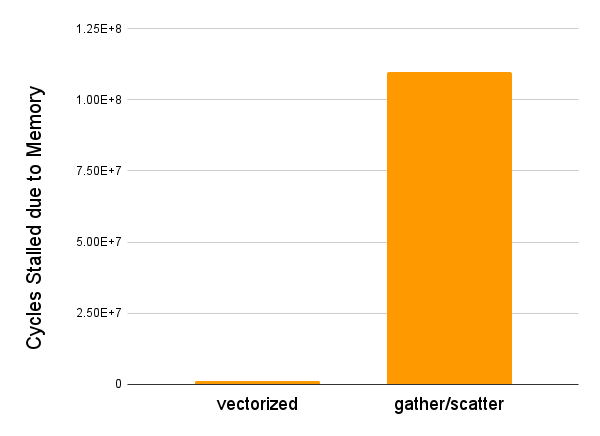
\includegraphics[width=0.5\textwidth]{img/gather_scatter_mem_stall.png}}\hfill
    \subfloat[Cycles with no instructions executed]{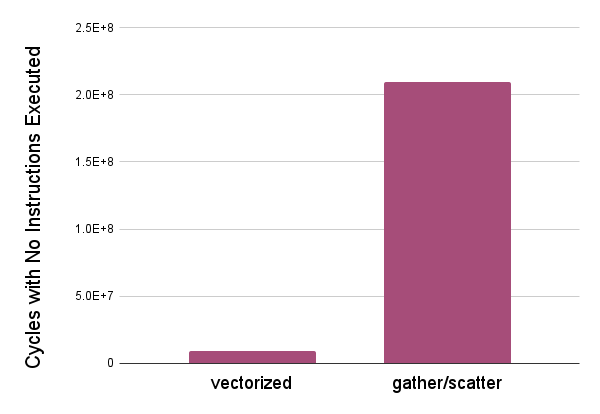
\includegraphics[width=0.5\textwidth]{img/gather_scatter_no_instr.png}}
    \caption{Comparing other metrics for vectorized code vs gather/scatter}
    \label{fig:four-images}
\end{figure}

The results of the experiment are presented in Figure [?]. The branch misses for the gather/scatter version are higher compared to the vectorized code. However, the total number of branch misses is very small, indicating that it may not have a significant impact on the overall performance. On the other hand, the cache misses, as shown in Figure [], are particularly interesting. It is observed that the use of gather loads and scatter stores has reduced the total number of cache misses. This observation may seem counter-intuitive given that we are accessing none-consecutive memory addresses however, since the memory addresses accessed through these instructions are very close to each other (stride distance of 2 in this case), it is likely that all the data needed can fit in a one or two cache lines, resulting in fewer cache misses.

The results presented in Figure [?] and [?] shed light on the significant performance degradation caused by the gather and scatter operations. The number of cycles that the processor has been stalled and has executed no instructions is increased by almost 10x due to the use of these instructions. This finding highlights the importance of caution when considering the use of gather and scatter operations in code optimization. While the reduction in cache misses may seem appealing, it is crucial to consider the potential impact on the overall performance of the code. Anypne deciding to use these gather and scatter instructions should carefully evaluate the trade-off between cache performance and the increased processor stall cycles caused by gather and scatter operations. Furthermore, it is recommended to perform thorough profiling and benchmarking of the code to ensure that the benefits outweigh the costs before implementing gather and scatter instructions in performance-critical sections of the code.








\section{ALC Strategies}

In this section we explain how we do the transformation for each case. We start by Wytte algorithm, show the potential cases where it would not result in good performance. Then we analyze what is happening in detail to fine the solution and propose our modified version which works well.


\section{Analysis Phase}

The analysis has three major roles:
\begin{enumerate}
    \item To make sure that for the given loop we are allowed to apply ALC.
    \item How does the structure of CFG look like and chooses the right approach for Apply ALC.
    \item Based on the information it gathers, is it benefitial to do the tranformation or not.
\end{enumerate}

As Wytte explained in his work, in order to be alowed to apply ALC which means that we need to make sure that the generated code will be correct and the result of the execution will be exactly the same as the result for exectuing scalar code, we must make sure that the loop has no function calls, no loop carried dependecy and there exists at least two paths inside the loop. The first responsiblity of the analysis is to check these restrictions.

Providing a general recipe to do the tranformations for any input code requires gathering infromation about exact structure of control flow, so that we can classify any sort of divergence in a pre-defined category. To attain this goal we first define three categories of divergence
which will cover all possible shapes of control flow. Having them classifed, we can then propose techniques and algorithms for applying ALC in each case. The three categories are followings:

\begin{enumerate}
    \item Single if statement.
    \item Single if-then-else statement.
    \item Any divergene with more that 2 control flow paths.
\end{enumerate}

There are different experimental factor that lead us to these three categories which include the level of difficulty to apply the pass and expected improvement for each case. The recipe to apply the transfromation on each case is explaned in next chapters.

Finally, After making sure that we are allowed to apply ALC and finding the right categoriy for the loop, we need to make the dicision of whether it's benefitial to do the tranformation or not. This is one the most challenging parts since the improvement that comes from the ALC depends on several different factors which some of them could be detected only at run time. In Section ?? we will explain these factors and requirements and how our cost model answers them in detail.   


\end{document}